% =====================================================================
% DRAFT RESULTS
%
% Numbers here come from paper/draft_results.txt and paper/tab_main.tex,
% both written by draft_results.py. Rerun that script and this section's
% table regenerates; the prose numbers marked with a comment need a
% manual pass.
%
% FIGURES: upload fig_method.png, fig_scale.png, fig_beforeafter.png and
% fig_difficulty.png into one folder in Overleaf, then add this to the
% preamble. Listing several paths means it works whether you name the
% folder figures, figs or figured, and also if the images sit at the
% project root.
%
%   \usepackage{graphicx}
%   \graphicspath{{figures/}{figs/}{figured/}{./}}
% =====================================================================

\section{Results}
\label{sec:results}

\subsection{Scale Predicts Bengali Reasoning; Pretraining Depth Does Not}
\label{sec:rq1}

Figure~\ref{fig:scale} is the central result. Plotting untuned accuracy against
parameter count separates the models cleanly into two regimes, and the
separating variable is not the one the field's Bengali-specific model releases
would predict.

\begin{figure}[htbp]
\centering
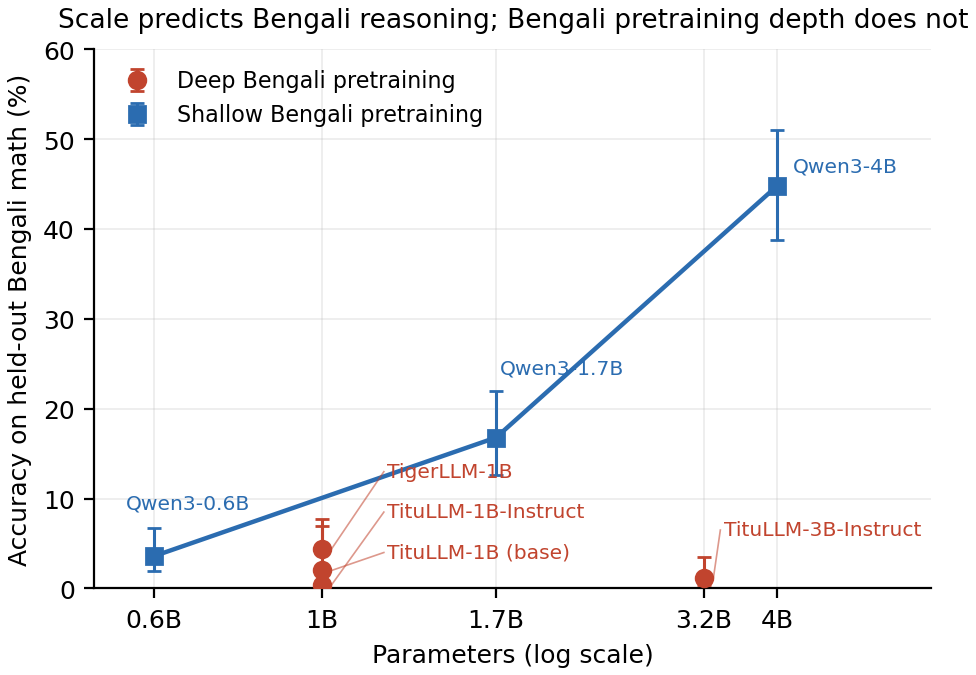
\includegraphics[width=\linewidth]{fig_scale.png}
\caption{Exact-match accuracy on held-out Bengali mathematics word problems,
plotted against total parameter count, for all seven backbones as released and
before any fine-tuning. Each model is scored on the same 250 items (100 for
TituLLM-1B base); vertical bars are Wilson 95\% intervals and the horizontal
axis is logarithmic. The line joins members of the Qwen3 family and is a visual
guide, not a fitted trend. Notice that the four models with deep Bengali
pretraining sit flat near the floor across a threefold range of parameters,
while the three with only incidental Bengali coverage climb steeply with
scale.}
\label{fig:scale}
\end{figure}

Within the Qwen3 family, which received no Bengali-specific pretraining beyond
whatever appears in a general multilingual mix, accuracy rises monotonically
and steeply: 3.6\% at 0.6B, 16.8\% at 1.7B, and 44.8\% at 4B. Every adjacent
step is significant under an unpaired Fisher exact test: $p=1.0\times10^{-6}$
from 0.6B to 1.7B, $p=1.3\times10^{-11}$ from 1.7B to 4B, and
$p=7.4\times10^{-30}$ across the full ladder. That is better than an order of
magnitude of improvement across less than one order of magnitude of
parameters.

The Bengali-specialised models show no such gradient. TituLLM-1B-Instruct
reaches 0.4\%, TituLLM-1B base 2.0\%, TigerLLM-1B 4.4\%, and TituLLM-3B-Instruct
1.2\%. Tripling the parameter count from 1B to 3.2B buys nothing. All four sit
inside each other's confidence intervals and all four sit near the floor.

The sharpest single comparison is TituLLM-3B-Instruct against Qwen3-1.7B.
TituLLM-3B-Instruct has roughly twice the parameters and was continually
pretrained on a large Bengali corpus with a tokenizer extended for the
language. Qwen3-1.7B has neither advantage. Qwen3-1.7B scores 16.8\% against
TituLLM-3B-Instruct's 1.2\% (Fisher exact, $p=1.7\times10^{-10}$). The
advantage is not an artifact of one difficulty tier. The smaller, Bengali-shallow model wins at easy (17.4\% against 1.4\%),
medium (20.3\% against 1.4\%), hard (13.4\% against 1.5\%) and olympiad (15.6\%
against 0.0\%) alike.

This answers RQ1 directly, and answers it in the negative. Targeted Bengali
pretraining depth, as delivered by the two publicly released Bengali model
families we could obtain, does not substitute for scale on mathematical
reasoning. Whatever those models gained from Bengali continued pretraining, and
they did gain something, since their tokenizers are far more efficient on
Bengali text, it did not transfer into mathematical competence.

\subsection{Minimal-Data Elicitation Moves No Model}
\label{sec:rq1b}

Table~\ref{tab:main} and Figure~\ref{fig:beforeafter} report the paired
before-and-after comparison for all seven backbones.

We report accuracy rather than precision, recall or F1 because the task is
free-form generation of a numeric answer scored by exact match, not
classification: there are no classes over which those metrics are defined and
no confusion matrix to construct. In their place we report the diagnostics that
do carry information for generative scoring, namely format-failure rate,
token-cap rate, language adherence, per-difficulty accuracy
(Table~\ref{tab:difficulty}) and answer retention
(Table~\ref{tab:retention}).

% Regenerate every table with:  python paper_stats.py
\begin{table*}[t]
\caption{Accuracy before and after LIMO-style fine-tuning on 873 curated
Bengali reasoning traces, on the same 250 held-out items per model
(TituLLM-1B base on 100). Intervals on each accuracy are Wilson 95\%.
$\Delta$ is the paired risk difference in percentage points with its 95\%
confidence interval; it is the effect size, and it is reported because a
$p$-value alone does not bound how large the change could be. $p$ is a
two-sided exact McNemar test on the discordant pairs. Notice that every
$\Delta$ interval contains zero.}
\label{tab:main}
\centering\small
\begin{tabular}{|l|c|c|c|c|c|c|c|c|}
\hline
\textbf{Model} & \textbf{Params} & \textbf{Bn depth} & \textbf{$n$} & \textbf{Before} & \textbf{After} & \textbf{$\Delta$ (pp)} & \textbf{95\% CI} & \textbf{$p$} \\
\hline
TituLLM-1B (base) & 1.0B & deep & 100 & 2.0\% & 0.0\% & -2.0 & [-4.7, +0.7] & 0.500 \\
TituLLM-1B-Instruct & 1.0B & deep & 250 & 0.4\% & 2.8\% & +2.4 & [+0.2, +4.6] & 0.070 \\
TigerLLM-1B & 1.0B & deep & 250 & 4.4\% & 2.4\% & -2.0 & [-4.8, +0.8] & 0.267 \\
TituLLM-3B-Instruct & 3.2B & deep & 250 & 1.2\% & 1.2\% & +0.0 & [-1.9, +1.9] & 1.000 \\
Qwen3-0.6B & 0.6B & shallow & 250 & 3.6\% & 6.0\% & +2.4 & [-0.7, +5.5] & 0.210 \\
Qwen3-1.7B & 1.7B & shallow & 250 & 16.8\% & 18.0\% & +1.2 & [-4.4, +6.8] & 0.780 \\
Qwen3-4B & 4.0B & shallow & 250 & 44.8\% & 39.6\% & -5.2 & [-13.0, +2.6] & 0.228 \\
\hline
\end{tabular}
\end{table*}

\begin{table*}[t]
\caption{Accuracy by difficulty tier, before and after fine-tuning, for
every backbone on the same held-out items. Tier counts are 69 easy, 69
medium, 67 hard and 45 olympiad for the models evaluated on 250 items,
and 30/24/29/17 for TituLLM-1B base on 100. Notice that the Qwen3
advantage holds in every tier rather than coming from one band, and that
no tier shows a consistent post-tuning gain.}
\label{tab:difficulty}
\centering\small
\begin{tabular}{|l|c|c|c|c|}
\hline
\textbf{Model} & \textbf{Easy} & \textbf{Medium} & \textbf{Hard} & \textbf{Olympiad} \\
\hline
TituLLM-1B (base) & 0.0 $\rightarrow$ 0.0 & 4.2 $\rightarrow$ 0.0 & 3.4 $\rightarrow$ 0.0 & 0.0 $\rightarrow$ 0.0 \\
TituLLM-1B-Instruct & 1.4 $\rightarrow$ 5.8 & 0.0 $\rightarrow$ 2.9 & 0.0 $\rightarrow$ 1.5 & 0.0 $\rightarrow$ 0.0 \\
TigerLLM-1B & 7.2 $\rightarrow$ 2.9 & 4.3 $\rightarrow$ 2.9 & 1.5 $\rightarrow$ 3.0 & 4.4 $\rightarrow$ 0.0 \\
TituLLM-3B-Instruct & 1.4 $\rightarrow$ 1.4 & 1.4 $\rightarrow$ 1.4 & 1.5 $\rightarrow$ 1.5 & 0.0 $\rightarrow$ 0.0 \\
Qwen3-0.6B & 2.9 $\rightarrow$ 8.7 & 4.3 $\rightarrow$ 4.3 & 4.5 $\rightarrow$ 9.0 & 2.2 $\rightarrow$ 0.0 \\
Qwen3-1.7B & 17.4 $\rightarrow$ 21.7 & 20.3 $\rightarrow$ 20.3 & 13.4 $\rightarrow$ 19.4 & 15.6 $\rightarrow$ 6.7 \\
Qwen3-4B & 59.4 $\rightarrow$ 55.1 & 44.9 $\rightarrow$ 34.8 & 40.3 $\rightarrow$ 40.3 & 28.9 $\rightarrow$ 22.2 \\
\hline
\end{tabular}
\multicolumn{1}{l}{\small All values are percentages, before $\rightarrow$ after.}
\end{table*}

\begin{figure}[htbp]
\centering
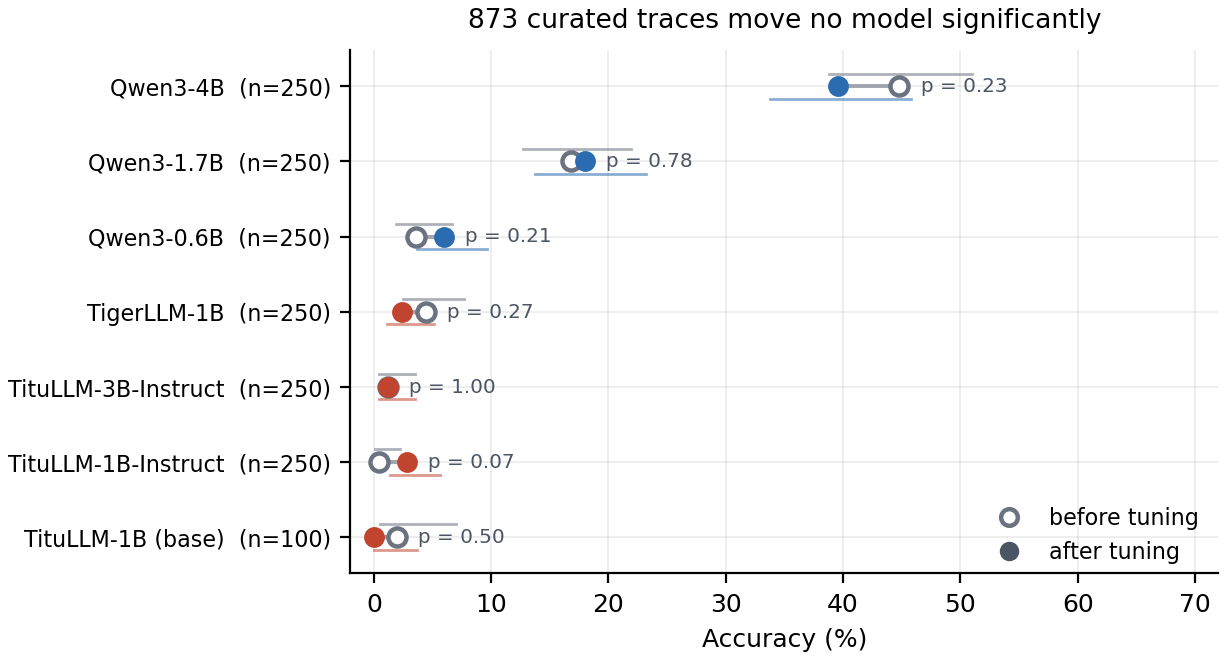
\includegraphics[width=\linewidth]{fig_beforeafter.png}
\caption{Exact-match accuracy for each backbone before and after LoRA
fine-tuning on the same 873 curated Bengali traces, scored on the same held-out
items in both conditions ($n=250$; $n=100$ for TituLLM-1B base). Hollow markers
are the untuned model, filled markers the adapter, and the thin lines behind
each marker are Wilson 95\% intervals. $p$ values are two-sided exact McNemar
tests on the discordant pairs. Notice that the intervals for the two conditions
overlap substantially for every model, and that no comparison crosses the 0.05
threshold.}
\label{fig:beforeafter}
\end{figure}

Not one of the seven comparisons reaches significance. The smallest $p$ value in
the table is 0.070, for TituLLM-1B-Instruct, on a change from 0.4\% to 2.8\%
that amounts to six additional correct answers out of 250. Three models moved
up, three moved down, and one did not move at all. That distribution is what
noise looks like.

The result is worth stating carefully, because a null result invites two
different readings and only one of them is supported here. The reading we can
defend is that 873 curated traces do not elicit latent mathematical reasoning
in Bengali at the 0.6B to 4B scale. The reading we cannot defend is that
LIMO-style elicitation does not work, full stop. Our largest model is 4B.
\textcite{wei2022emergent} place the threshold for arithmetic emergence near
13B and for chain-of-thought benefit substantially higher, and every model in
this study sits below both. A negative result collected entirely below a
capability threshold is evidence about that region, not about the method.

Qwen3-4B is the one row where the point estimate moved by a visible margin, from
44.8\% down to 39.6\%. The direction survived the extension from 100 items to
250, but the significance did not arrive with it: 56 items were lost against 43
gained, giving $\Delta = -5.2$ percentage points with a 95\% confidence interval
of $-13.0$ to $+2.6$, and an exact McNemar $p=0.228$. The interval contains zero
and is wide enough to accommodate a modest gain, so we do not read a real
degradation into it. It is worth noting that this is the only model with
enough baseline accuracy for a degradation to have been visible at all.

\subsection{Output Behaviour Changed Even Though Accuracy Did Not}
\label{sec:behaviour}

The tuning was not inert. It changed what the models produced; it simply did not
change whether the produced answers were right.

The clearest case is TituLLM-1B base. Untuned, it hit the generation cap on
100\% of items, meaning it never once emitted a stop token and every completion
was truncated at the token budget. After fine-tuning on 873 traces, that fell to
47\%. The model learned, from a very small number of examples, what a finished
Bengali reasoning trace looks like and when to stop producing one. Its accuracy
over the same items went from 2.0\% to 0.0\%.

Across the other backbones the cap rate mostly moved the other way. It rose
after tuning for four of the seven models, most sharply for Qwen3-0.6B (4.8\%
to 36.8\%) and TituLLM-3B-Instruct (8.0\% to 29.2\%). Trained on long worked
solutions, those models produced longer outputs. They did not produce more
correct ones. Qwen3-4B is the informative exception: the one model with real
baseline competence barely moved on this measure at all, from 8.8\% to 7.6\%,
which is what we would expect from a model that already knew how to finish a
worked solution before it saw any of ours.

Stopping behaviour, then, moved in whichever direction the base model had the
most room to move in, and in no case did it move accuracy with it. The next
section takes this further and asks what the adapter changed at the level of
individual items.

\subsection{What the Fine-Tuning Actually Did}
\label{sec:retention}

A null result invites the objection that nothing happened at all: that the
adapter never took, or that LoRA at rank 16 is too small to move a model. The
item-level data rules that out. A great deal happened. It simply was not
learning to reason.

Table~\ref{tab:retention} reports answer retention, meaning the share of items
a model answered correctly before fine-tuning that it still answered correctly
afterwards. If 873 traces were teaching mathematical reasoning, retention
should be high and the gains should sit on top of it. That is not the pattern.

\begin{table}[htbp]
\caption{Answer retention. Of the items each model answered correctly
before fine-tuning, how many it still answered correctly afterwards, and
how many items changed outcome in either direction. Notice that no model
retained even half of what it already knew, which is why the small net
changes in Table~\ref{tab:main} understate how much the adapter moved.}
\label{tab:retention}
\centering\small
\begin{tabular}{|l|c|c|c|c|}
\hline
\textbf{Model} & \textbf{Correct before} & \textbf{Retained} & \textbf{Retention} & \textbf{Items flipped} \\
\hline
Qwen3-4B & 112 & 56 & 50\% & 99 / 250 \\
Qwen3-1.7B & 42 & 18 & 43\% & 51 / 250 \\
Qwen3-0.6B & 9 & 4 & 44\% & 16 / 250 \\
TigerLLM-1B & 11 & 2 & 18\% & 13 / 250 \\
TituLLM-3B-Instruct & 3 & 0 & 0\% & 6 / 250 \\
TituLLM-1B-Instruct & 1 & 0 & 0\% & 8 / 250 \\
\hline
\end{tabular}
\end{table}

Qwen3-4B answered 112 items correctly before tuning and kept 56 of them. It
also answered 43 items correctly that it had failed before. In total 99 of 250
items changed their outcome, close to 40\% of the evaluation set, while net
accuracy moved by 13 items. The same shape holds down the scale: no model
retained even half of what it already knew. The adapter did not add a layer of
competence on top of the base model. It substantially rewrote which problems
the model could solve, and the replacement set happened to be slightly worse
than the original.

The mechanism is visible in the generated text. Before fine-tuning, Qwen3-4B
closed 225 of 250 completions with the Bengali word for ``answer'' followed by
its result, a convention it adopted on its own, since the evaluation prompt
asks only that the model answer in Bengali and specifies no format. After
fine-tuning it did so on 3 of 250. In its place the model adopted the format of
the training corpus: Ganit's traces are written as a \texttt{<think>} block
followed by an \texttt{<answer>} block, and after tuning every one of the 250
completions opened a \texttt{<think>} block. Median output length fell from
1,046 tokens to 887, the proportion of Bengali characters fell from 87.0\% to
82.0\%, and the number of explicit step markers roughly halved.

This is the Superficial Alignment Hypothesis \parencite{zhou2023lima} observed
from the unfavourable side. In LIMA's setting a small number of examples
exposes capability the pretrained weights already hold, and the result is a
useful model. Here the same small number of examples reshaped format, length,
language mix and stopping behaviour just as comprehensively, and exposed
nothing, because at this scale there was little underneath to expose. Style
transferred completely. Reasoning did not transfer at all.

\subsubsection*{A sensitivity check on the format change}

Because the output format changed, it is worth confirming that the accuracy
drop is not an artifact of answer extraction. Our scorer looks for an
\texttt{<answer>} block first, then a boxed expression, then the Bengali answer
marker, and only if none of those are present does it fall back to taking the
last number in the completion. After fine-tuning, 230 of 250 Qwen3-4B
completions contained a well-formed \texttt{<answer>} block and were therefore
parsed by the strongest branch of the extractor. The remaining 20 exhausted the
generation budget inside the \texttt{<think>} block and were scored by the weak
fallback. Of the 56 items Qwen3-4B lost, 45 produced a well-formed
\texttt{<answer>} that was simply wrong. The failures are arithmetic, not
formatting. On one item with gold answer 16 the tuned model emitted
\texttt{<answer>0</answer>}; on another with gold 126 it emitted
\texttt{<answer>14</answer>}. In both cases the extractor read exactly what the
model wrote.

To bound the effect, we recomputed accuracy crediting every fallback-scored
item as correct, which is the most generous assumption available. Post-tuning
accuracy under that assumption is 46.8\%, against a measured 39.6\% and a
pre-tuning 44.8\%. The true value therefore lies somewhere between a loss of
5.2 points and a gain of 2.0 points. We cannot sign the effect, which is
consistent with the exact McNemar test returning $p=0.228$, and the substantive
conclusion is unchanged in either direction: 873 curated traces did not produce
a detectable improvement in Bengali mathematical reasoning at this scale.

\subsection{The Null Is Not a Difficulty-Calibration Artifact}
\label{sec:difficulty}

The most obvious objection to Section~\ref{sec:rq1b} is that our training set was
simply too hard. The LIMO window selects problems a 32B model solves between 1
and 16 times out of 32, which for a 1.7B model may be far outside the range it
can learn anything from. If so, the null would say more about our data selection
than about elicitation.

We tested this directly. Holding the backbone, the LoRA configuration, the seed,
the prompt and the evaluation items constant, we built a second training set of
1,000 traces from the opposite end of the difficulty distribution, requiring at
least 28 correct out of 32, and trained the same Qwen3-1.7B on it.

\begin{figure}[htbp]
\centering
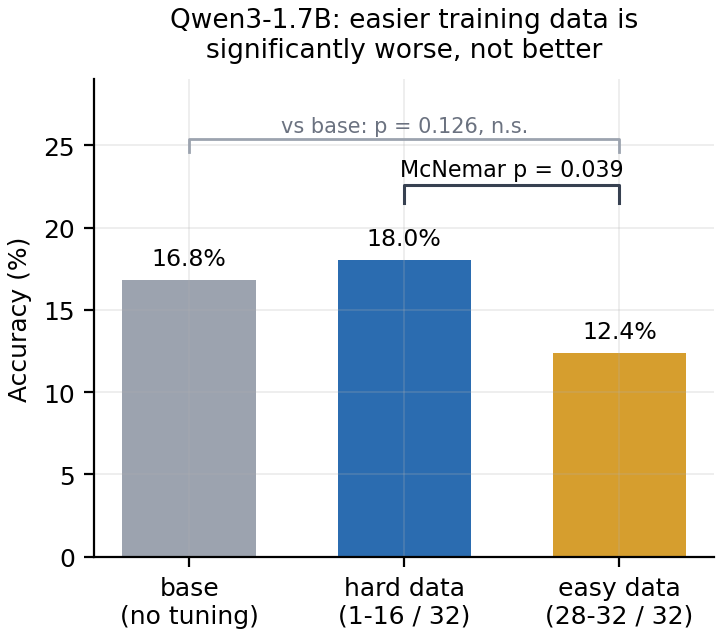
\includegraphics[width=0.72\linewidth]{fig_difficulty.png}
\caption{Qwen3-1.7B under three conditions, scored on the same 250 held-out
items, with backbone, LoRA configuration, seed, prompt and evaluation items
held fixed so that training-data difficulty is the only thing that varies. The
easy-data adapter is significantly worse than the hard-data adapter (exact
McNemar, $p=0.039$); against the untuned base it is lower but not significantly
so ($p=0.126$), as marked. Notice that easier, better-calibrated training data
did not rescue the null result and if anything moved accuracy the wrong way.}
\label{fig:difficulty}
\end{figure}

The easy-data adapter reached 12.4\%, against 18.0\% for the hard-data adapter
and 16.8\% for the untuned base. The gap between the two adapters is
significant (exact McNemar, 27 items lost against 13 gained, $p=0.039$), and it
runs in the opposite direction to the objection. Easier, better-calibrated
training data did not rescue the null. It made results worse.

Against the untuned base, by contrast, the easy-data adapter is lower but not
significantly so (12.4\% against 16.8\%, exact McNemar $p=0.126$). The claim we
can defend is the narrower one: easier data is significantly worse than harder
data, not that it is significantly worse than no tuning at all.

This closes the difficulty explanation. The models can learn from calibrated
data, and doing so does not improve held-out reasoning and may actively harm it.

\subsection{The Bengali Tokenizer Tax}
\label{sec:tokenizer}

One finding did come out clearly in favour of the Bengali-specialised models,
and it is a real one even though it did not translate into accuracy.
Table~\ref{tab:tokenizer} reports token counts for the same 873 training
traces under each tokenizer.

Qwen3 needs roughly $3.1\times$ more tokens than TituLLM to represent identical
Bengali text, close to the $3.5\times$ reported by
\textcite{yong2025crosslingual} and consistent with the per-model premiums in
\textcite{petrov2023language}.

The cost is concrete rather than theoretical. On a single 16GB consumer card it
determined which configurations were trainable at all. Qwen3-4B could not be
trained at a 4,096-token sequence limit and required a reduction to 2,048, which
truncated 104 of the 873 traces. No Bengali-tokenized model faced that
constraint. The same pressure appeared at inference: TituLLM-3B-Instruct pairs
3.2B parameters with a 170,497-token vocabulary, which makes the output logits
tensor the binding memory cost during generation and forced a batch size of one.

It is worth noting that TigerLLM's efficiency is inherited rather than earned.
Gemma3 ships a 262k vocabulary described as balanced for non-English languages
\parencite{gemma3}, and TigerLLM adds exactly one token to it. TituLLM, by
contrast, extended Llama-3.2's vocabulary deliberately for Bengali. Both end up
around three times more efficient than Qwen3 on this corpus, by quite different
routes.

The broader point is that tokenizer efficiency and downstream reasoning are
separable. The two most token-efficient models in this study are also the two
weakest at mathematics. Efficiency on Bengali text is necessary for practical
deployment on constrained hardware, and it is not sufficient for reasoning.
